\chapter{Appendix}

\newpage
\section{Full Inverse Kinematics Expressions}
\label{app:ik}

{\footnotesize\begin{align}
    q_1 &= \operatorname{atan2}(y_d, x_d)
    \\[3ex]
    q_2 &= \operatorname{acos}\left(\frac{a_2^2 - a_3^2 + \left(\sqrt{x_d^2 + y_d^2} - a_1\right)^2 + (d_b - z_d)^2}
    {2 \cdot a_2 \cdot \sqrt{\left(\sqrt{x_d^2 + y_d^2} - a_1\right)^2 + (d_b - z_d)^2}}\right) -
    \operatorname{atan2}\left((d_b - z_d), \left(\sqrt{x_d^2 + y_d^2} - a_1\right)\right)
    \\
    q_3 &= \operatorname{acos}\left(\frac{a_2^2 + a_3^2 - \left(\sqrt{x_d^2 + y_d^2} - a_1\right)^2 - (d_b - z_d)^2}
    {2 \cdot a_2 \cdot a_3}\right)
    \label{eqn:inverse_kinematics}
\end{align}}


\newpage
\section{Servo Module Schematic}
\label{app:pcb}

\begin{figure}[htb]
    \centering
    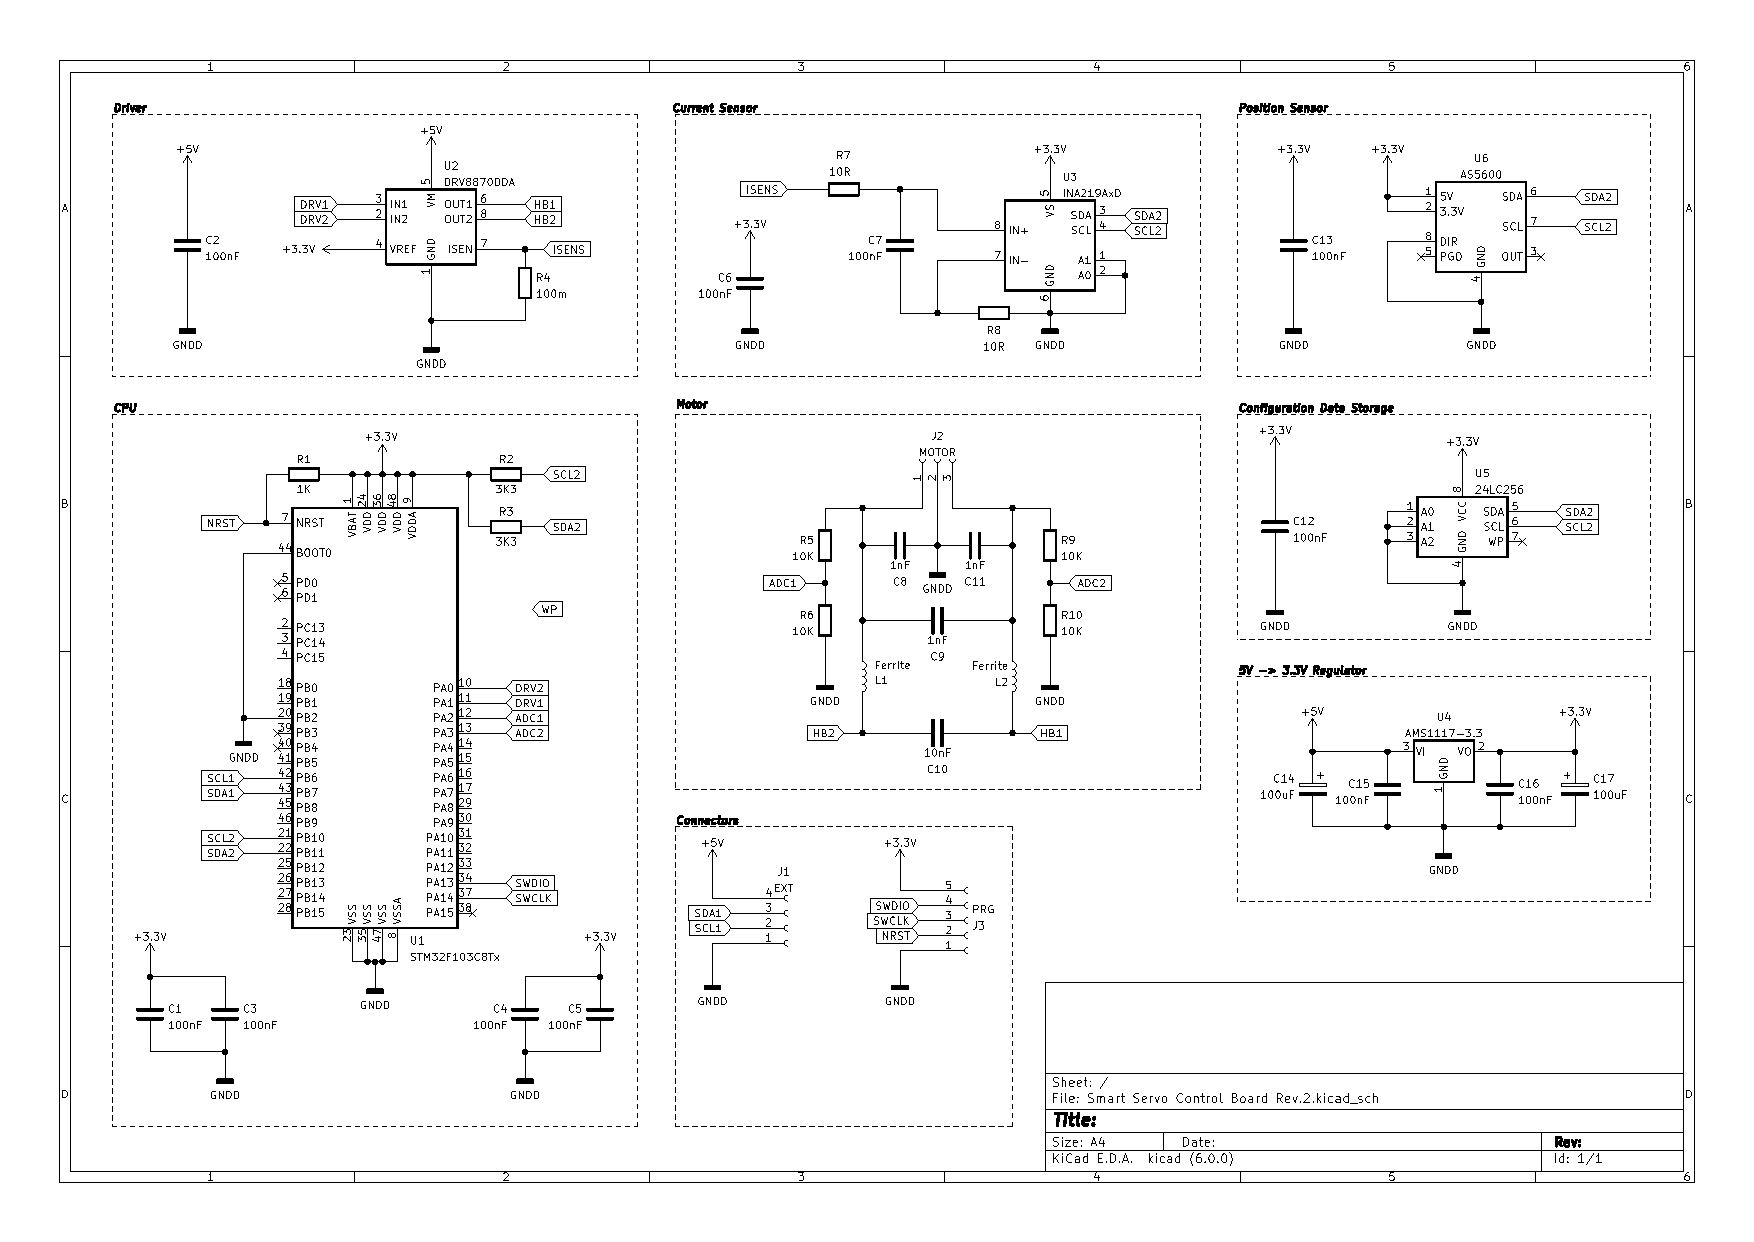
\includegraphics[angle = 90, width=0.8\textwidth]{images/schematic.pdf}
\end{figure}


\newpage
\section{Software Architecture}
\label{app:software}

\begin{figure}[htb]
    \centering
    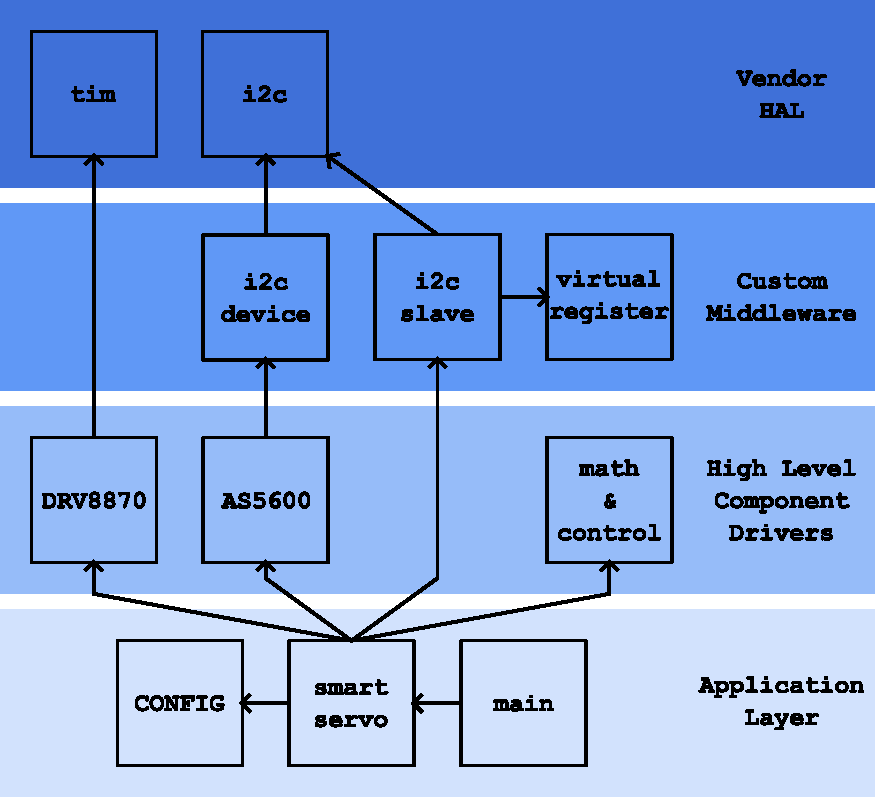
\includegraphics[width=\textwidth]{images/software_architecture.pdf}
\end{figure}


\newpage
\section{Register Map}
\label{app:register}

\begin{longtable}{@{} l l l l l @{}}
\caption{System Register Map} \\

% --- Intestazione Prima Pagina ---
\toprule
\textbf{Addr} & \textbf{Register Name} & \textbf{Data Type} & \textbf{Group} & \textbf{Default} \\
\midrule
\endfirsthead

% --- Intestazione Pagine Successive ---
\toprule
\textbf{Addr} & \textbf{Register Name} & \textbf{Data Type} & \textbf{Group} & \textbf{Default} \\
\midrule
\endhead

% --- Footer Pagine Intermedie ---
\midrule
\multicolumn{5}{r}{\textit{Continued...}} \\
\bottomrule
\endfoot

% --- Footer Finale ---
\bottomrule
\endlastfoot

% --- CONTENUTO ---

% SW-PID Controller (Tipi dedotti da DefaultSettings: float)
\texttt{0x00} & ProportionalGain   & \texttt{float}    & SWPID Control & $10.0f$ \\
\texttt{0x01} & IntegralGain       & \texttt{float}    & SWPID Control & $0.9f$ \\
\texttt{0x02} & DerivativeGain     & \texttt{float}    & SWPID Control & $0.1f$ \\
\texttt{0x03} & AntiwindupMax      & \texttt{float}    & SWPID Control & $5.0f$ \\
\texttt{0x04} & AntiwindupMin      & \texttt{float}    & SWPID Control & $-5.0f$ \\
\texttt{0x05} & OutputMax          & \texttt{float}    & SWPID Control & $1.0f$ \\
\texttt{0x06} & OutputMin          & \texttt{float}    & SWPID Control & $-1.0f$ \\
\addlinespace

% Servo Motor State (Non presenti in Default, ipotizzo float per coerenza)
\texttt{0x20} & DesiredPosition    & \texttt{int32\_t}  & Servo State & 0 \\
\texttt{0x21} & ActualPosition     & \texttt{int32\_t}  & Servo State & - \\
\texttt{0x22} & PositionOffset     & \texttt{int32\_t}  & Servo State & -2048 \\
\texttt{0x26} & DutyCycle          & \texttt{int32\_t}  & Servo State & - \\
\addlinespace

% AS5600 (Tipi dedotti: uint16_t)
\texttt{0x40} & ZeroPosition       & \texttt{uint16\_t} & AS5600     & \texttt{0x000} \\
\texttt{0x41} & StopPosition       & \texttt{uint16\_t} & AS5600     & \texttt{0xFFF} \\
\addlinespace

\end{longtable}


\newpage
\section{Metrics Formulae}
\label{app:metrics}

\textbf{Root Mean Square Error (RMSE)}
$$\text{RMSE} = \sqrt{ \frac{1}{N} \sum_{i=1}^{N} \left( y_{meas}[i] - y_{ideal}[i] \right)^2 }$$

This metric quantifies the standard deviation of the residuals between the measured output ($y_{meas}$) and the ideal
theoretical reference ($y_{ideal}$). It serves as the primary indicator of the system's overall linearity accuracy,
aggregating the error over the entire dataset.


\textbf{Maximum Absolute Error}
$$E_{max} = \max_{i} \left| y_{meas}[i] - y_{ideal}[i] \right|$$

Represents the worst-case deviation observed across the entire operating range. It identifies the single instance
where the actuator's position diverged most significantly from the expected ideal value.


\textbf{Hysteresis Loop Area}
$$\mathcal{A}_{hyst} = \left| \int_{x_{min}}^{x_{max}} \left( y_{fwd}(x) - y_{bwd}(x) \right) \, dx \right|$$

Calculated via numerical integration (trapezoidal rule), this value represents the total area enclosed between the
forward ($y_{fwd}$) and backward ($y_{bwd}$) trajectories. It quantifies the cumulative effect of mechanical backlash,
friction, and sensor noise over a full motion cycle.


\textbf{Average Hysteresis Error}
$$H_{avg} = \frac{\mathcal{A}_{hyst}}{x_{max} - x_{min}}$$

This metric normalizes the hysteresis area by the input signal range ($x_{max} - x_{min}$). It provides the average
magnitude of the hysteresis gap in degrees, allowing for a direct and fair comparison between systems operating on
different input domains.


\newpage
\section{Bill of Material}
\label{app:bom}

Bill of Materials (BOM) for a single custom actuator module. Prices reflect the per-unit cost derived from bulk purchases
on third-party websites and are comprehensive of shipping.

\begin{table}[htbp]
    \centering
    \begin{tabular}{lccc}
        \toprule
        \textbf{Component}  & \textbf{Qty} & \textbf{Bulk Price Reference} & \textbf{Unit Cost (€)} \\
        \midrule
        Custom PCB                              & 1             & 6.18€ / 10 pcs    & 0.62 \\
        STM32F103C8T6 (MCU)                     & 1             & 7.99€ / 10 pcs    & 0.80 \\
        AS5600 (Magnetic Sensor)                & 1             & 4.42€ / 5 pcs     & 0.88 \\
        DRV8870 (Motor Driver)                  & 1             & 2.20€ / 10 pcs    & 0.22 \\
        Tantalum Cap. (100 $\mu$F)              & 2             & 1.47€ / 10 pcs    & 0.29 \\
        AMS1117 (LDO Regulator)                 & 1             & 2.16€ / 50 pcs    & 0.04 \\
        SMD Passives (0603 R/C)                 & $\approx$30   & Lump sum          & 0.25 \\
        MG996R Servo Motor\textsuperscript{*}   & 1             & 20.39€ / 5 pcs    & 4.08 \\
        \midrule
        \textbf{Total Cost per Module} & & & \textbf{7.18} \\
        \bottomrule
    \end{tabular}
    \vspace{1ex}

    {\footnotesize \textsuperscript{*}Current market price (2025). Using older stock (2018), the motor unit cost was
    $\approx 1.92$€, lowering the total to $\approx 5.02$€.}
\end{table}
